\documentclass[10pt,twocolumn]{article} 

% use the oxycomps style file
\usepackage{oxycomps}

% use packages for timeline
\usepackage{array, booktabs, longtable}
\usepackage{graphicx}
\usepackage[x11names, table]{xcolor}
\usepackage{caption}
\usepackage[most]{tcolorbox}
\DeclareCaptionFont{blue}{\color{LightSteelBlue3}}

\newcommand{\foo}{\color{LightSteelBlue3}\makebox[0pt]{\tiny\textbullet}\hskip-0.5pt\vrule width 1pt\hspace{\labelsep}}
\newcommand{\bfoo}{\raisebox{2.1ex}[0pt]{\makebox[\dimexpr2\tabcolsep]%
{\color{LightSteelBlue3}\tiny\textbullet}}}%
\newcommand{\tfoo}{\makebox[\dimexpr2\tabcolsep]%
{\color{LightSteelBlue3}$\boldsymbol \uparrow $}}%

% read references.bib for the bibtex data
\bibliography{references}

% include metadata in the generated pdf file
\pdfinfo{
    /Title (The Occidental Computer Science Comprehensive Project: Predicting Cryptocurrency Prices for Index Fund Rebalancing)
    /Author (Odelia Putterman)
}

% set the title and author information
\title{The Occidental College Computer Science Comprehensive Project Proposal: \\ Predicting Cryptocurrency Prices for Index Fund Rebalancing}
\author{Odelia Putterman}
\affiliation{Occidental College}
\email{putterman@oxy.edu}

\begin{document}

\maketitle

\begin{abstract}
This paper is the final paper outlining my Occidental College Computer Science Comprehensive Project (COMPs): \textit{Predicting Cryptocurrency Prices for Index Fund Rebalancing}. This paper begins by introducing this project's problem context. Next, it address the technical aspects of realizing this work. This paper also addresses lingering ethical concerns. Replication instructions and an overview of the code developed in this work for future users to engage with this project have been included as GitHub README documents in addition.
\end{abstract}

\section{Problem Context} \label{problemcontext}

Investing is a means by which people can grow their money exponentially, but it also holds the potential for significant loss, especially in the context of day trading.

\subsection{Index Funds: Explained}

As it stands, it's difficult, if not entirely impossible, to predict the exact performance of individual stocks. Accordingly, people invest in index funds: collections of stocks which follow some set of rules for construction. Index funds mirror the whole market rather than a particular holding, with funds mutually pooled (i.e. the stock holdings shared across many holders). Money that goes into an index fund is invested in all the stocks the fund holds, growing the diversification of the fund and minimizing its dependence on individual stock performance. Further, index funds are periodically re-balanced to offset losses and risk, and companies are sold once they leave these predefined rules or parameters discussed.

\subsection{Cryptocurrencies: Unique Opportunity and Approach}

Index funds are generally constructed using fundamental measures of a company (aka fundamentals), such as cash flow, sales, and dividends. However, cryptocurrencies have none of these intrinsic metrics. The cryptocurrencies themselves are a currency rather than a materialized product, so there are no sales or dividends to be found; their only true measure is price. Accordingly, any approach to creating and maintaining a cryptocurrency index fund must be revolutionary in nature.

Cryptocurrencies are incredibly volatile, making re-balancing especially important. Their instability also offers a unique opportunity for leveraging their turning points to optimize gains if high-accuracy price prediction can be achieved. If we could predict cryptocurrency prices in advance, we could leverage this knowledge to maximize gains while keeping a sense of security with the breadth of the fund.

Typically, index funds are re-balanced on a consistent, preset schedule, such as the third Friday at the end of each calendar quarterly. But, what if we could predict cryptocurrency prices to decide how and when to re-balance such a cryptocurrency fund instead? If this succeeded, the results would be revolutionary in nature and a first-of-its-kind for maintaining a balanced, high-return cryptocurrency fund.

People have previously attempted to predict the behavior of cryptocurrencies with some success, as discussed below in \nameref{priorwork}. I aim to follow in their steps with a slightly different approach and following implementation.

\section{Technical Background} \label{technicalbackground}

Here, I introduce the technical background required to fully comprehend the methods this project undertakes.

\subsection{What Are Cryptocurrencies?}

This project involves cryptocurrencies, a relatively new phenomena stemming from advances and uses of blockchain technologies. Cryptocurrencies were first created for their supposed safety and security arising from their basis in blockchain technology. According to \textcite{WhatIsBlockchain}, ``Blockchain is a shared, immutable ledger that facilitates the process of recording transactions and tracking assets in a business network". Each transaction is recorded as a ``block" of data, connected to the blocks before and after it in an irreversible chain (aka a blockchain).

\subsection{Sentiment Data and Sentiment Analysis}

Sentiment data is essentially the same as it sounds: data which signifies sentiment. Sentiment analysis, similarly, is the use of computational algorithms to study subjective information (i.e. sentiment). It is particularly important for understanding the social sentiment of a given thing \cite{SentimentAnalysisConcept}. In the context of this project, the sentiment data is data which can be analyzed to search for crowd feelings on cryptocurrencies, while the sentiment analysis is the analysis of this data to learn attitudes towards cryptocurrencies.

\subsection{Long Short-Term Neural Networks} \label{longshorttermneuralnetworks}

Long short-term neural networks (LSTMs) are a type of neural network or, more specifically, recurrent neural network (RNN), capable of long short-term predictions.

\begin{figure}
    \centering
    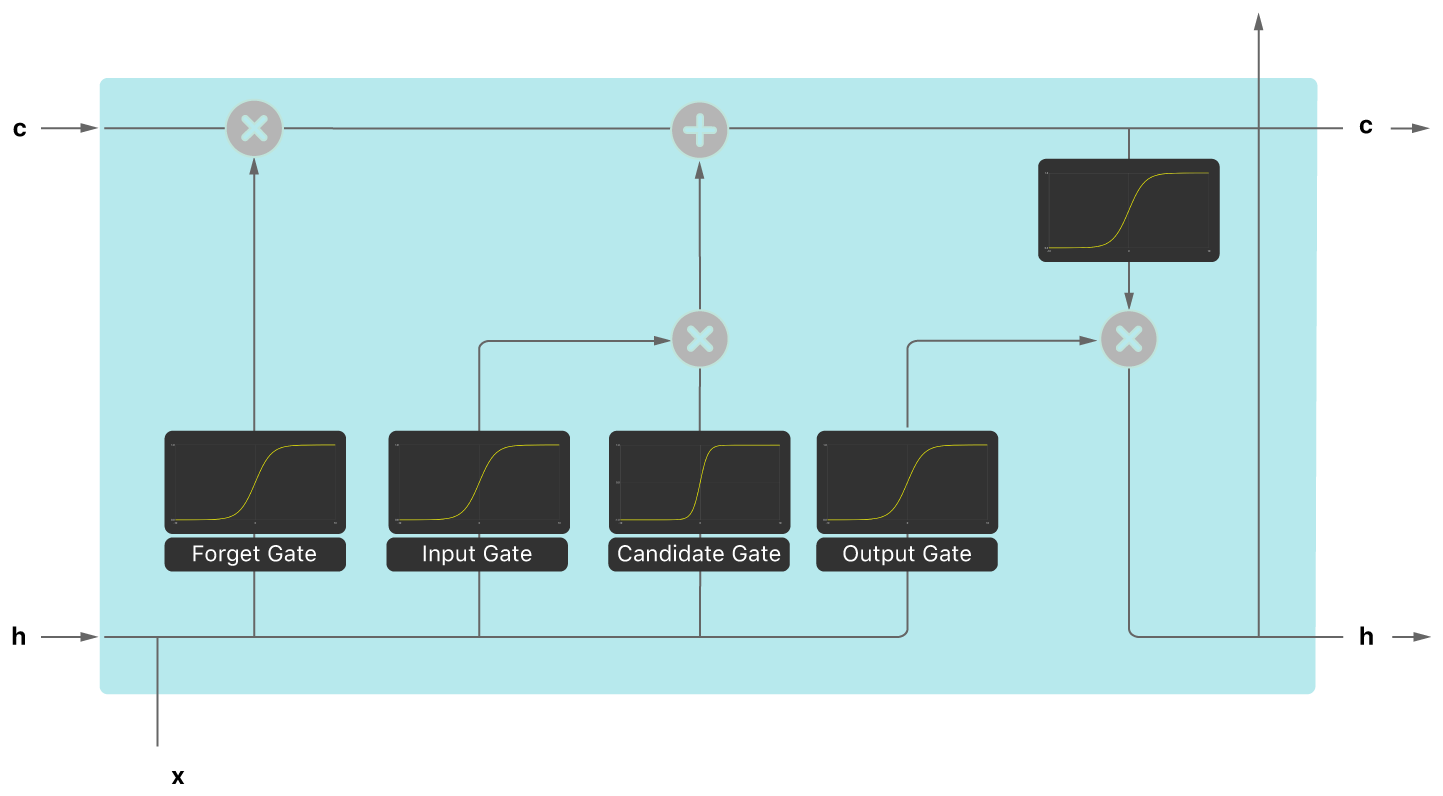
\includegraphics[scale=0.15]{images/four_layers.png}
    \caption{
        Sketch of the four gates composing LSTMs and their connections. From \textcite{apple}.
    }
    \label{lstm-four-layers}
\end{figure}

\subsubsection{Recurrent Neural Networks}

RNNs are a type of neural network capable of learning order dependence, which is key in sequence prediction problems. They differ from traditional feedforward neural networks, or multilayer perceptrons (MLPs), in their inclusion of feedback connections. To be an RNN, a system must:

\begin{enumerate}
    \item Be able to store information for an arbitrary period
    \item Be resistant to noise (i.e. random inputs, outliers, etc.).
    \item Have trainable system parameters.
\end{enumerate}

In RNNs, the \emph{context} is learned, meaning an RNN contains cycles which feed the network outputs, or activations, from a prior time step as input to the network for future time steps. However, they fail to ``remember" things from far back -- RNNs are susceptible to backpropagated error. These neural networks have hidden layers which can decay or blow up when circling around a feedback connection \cite{GentleIntroductionToLSTMNetworks}. Essentially, layers in RNNs with small enough gradient updates stop learning, usually in relatively early-on layers, causing short-term memory, or what is known as the \textit{vanishing gradient problem}, while layers with large enough gradients exponentially grow towards infinity, causing a blow-up problem and an unrealistic expectation for reliance on unimportant, or not as important as is implied, information \cite{IllustratedGuideToLSTMs}.

\subsubsection{LSTM Motivation}

LSTMs are a subset of recurrent neural networks (RNNs) similar, in most respects, to RNNs. They were first introduced in 1997 by Hochreiter and Shmidhuber \cite{UnderstandingLSTMs}. LSTMs differ from RNNs in their ability to solve the vanishing gradients and exploding gradients problems. Like RNNs, they learn order dependence in sequence prediction problems, only they are far more effective at retaining both long-term and short-term memory. They can keep information about the past for a unfixed period, to be decided by the input data weights as feedback connections are formed throughout the neural network operations; they use contextual information flexibly. LSTMs can traverse longer time steps to store important information with a constant error flow, avoiding the RNN problem of exponential blowing-up and decay \cite{GentleIntroductionToLSTMNetworks}. These feedback connections, or loops, allow for the persistence of information in traditional RNNs and, correspondingly, LSTMs. RNNs and LSTMs can be thought of as multiple copies of the same network, each passing information to the succeeding network. When the gap in knowledge from the prior input information to the next is relatively small, an RNN may succeed. But substantial research shows LSTMs far outperform typical RNNs when more context is needed \cite{UnderstandingLSTMs}.

\subsection{Index Fund Rebalancing}

Index fund rebalancing is the process of selling and buying stocks to balance the distribution across an index fund. There are many ways to re-balance an index fund. The usual choice is \textbf{calendar rebalancing}. In calendar rebalancing, the index fund holdings are reviewed on a preset calendar basis and adjusted to their original form. The actual rebalancing is done by examining issues such as transaction costs and drifts. Another type of rebalancing, later discussed, is \textbf{percentage-of-portfolio rebalancing}. According to \textcite{TypesOfRebalancingStrategies}, percentage-of-portfolio rebalancing is a ``rebalancing schedule focused on the allowable percentage composition of an asset in a portfolio. Every asset class, or individual security, is given a target weight and a corresponding tolerance range." There are many other types of rebalancing algorithms, but these are the two most important rebalancing algorithms to understand for the scope of this project.

\section{Prior Work} \label{priorwork}

LSTMs are one of the most widely employed methods for sequential data problems and time-series forecasting. In this section, we will focus on prior work in using LSTMs for stock price prediction and examine existing index fund rebalancing algorithms.

\subsection{Sentiment Analysis}

According to efficient market hypothesis, stock prices are driven by news rather than past and present prices -- they change based on news of changing fundamentals and human psychology (investor reactions to this news) \cite{LSTMSentimentAnalysis}. This suggests our input data to an LSTM for stock price predictions should include fundamentals and sentiment analysis so we can model prices based on changes in news and sentiment which gauge crowd feelings towards a given stock or industry.

\textcite{ReviewAndTaxonomyOfPredictionTechniques} recently employed fundamental analysis for stock price prediction, analyzing company profiles, industry, politics, the economy, and social media according to \textcite{LSTMSentimentAnalysis}. However, as \textcite{LSTMSentimentAnalysis} mention, this type of fundamental data is usually rather abstract or unstructured, making it hard to fit into a form LSTMs can use. Instead, \textcite{LSTMSentimentAnalysis} suggest using NLP methods to distill relevant information. Sentiment analysis is a strong candidate currently used to analyze text for emotional sentiments and reactions to ``understand" human feeling. From this ``understanding", we can examine how a stock may perform based on human feelings towards this stock. If, for example, negative sentiment about bitcoin is spreading, this may signal to us a coming drop in the bitcoin stock price. As such, sentiment analysis of crowd psychology can monitor public opinion \cite{LSTMSentimentAnalysis}.

\subsection{RNNs and LSTMs} \label{RNN-LSTMs}

RNNs, particularly their LSTM derivative, have been shown to outperform traditionally used models, such as support vector machines (SVMs), in accurately predicting values for time-series problems \cite{LSTMSentimentAnalysis}. By feeding a combination of fundamental and sentiment analysis to LSTMs to analyze, researchers have made promising strides towards success in predicting stock prices.

\textcite{LSTMSentimentAnalysis} used a long short-term memory neural network with text sentiments and historical stock transactions to predict stock prices similar to my approach for this project. The authors argued in the paper's introduction for the importance of aggressive investing strategies and, hence, the usefulness of accurate stock trend forecasting. They used fundamental analysis and technical analysis to forecast stock prices in addition to an LSTM, which was applied to this forecasting. Using text sentiment from blog articles, social media, online forum posts, and product reviews, the authors aimed to understand online public opinions. They used an existing NLP algorithm (BERT) to classify the texts into sentiment categories by counting the emotional words that appeared in a given sentence, after which they calculated a score for each emotional word, and, with these individual scores, outputted the condition of the sentence. Further, this article addressed pre-processing data to get it into a form where it can be passed to the related ML algorithm, which was very useful for me in learning how to apply my project's own product algorithm.

\subsection{Other Models}

\textcite{ForecastingAndTradingCryptoWithML} examined the predictability of three major crypto contenders: Bitcoin, Ethereum, and Litecoin. They focused on times of extreme upheaval and used linear models, random forests, and support vector machines for their predictive work. Of the 18 models they built, 13 models had a success rate over 50\%, affirming the promise of ML algorithms for cryptocurrency stock price prediction. In their introduction, they explained the proposal of sentiment analysis for stock price prediction, which is what motivated me to choose the same for my project.

\subsection{Trading Algorithms}

There are many possible trading algorithms to use for index fund rebalancing. 

\subsubsection{Mean-Variance Optimization}

One such trading algorithm is mean-variance optimization. \textcite{MeanVarianceAlgorithmicTrading} implores this algorithm, implementing Markowitz's portfolio optimization (MPT) and the Modern Portfolio Theory in python as trading strategies with the \textit{zipline} library. The general goal of MPT is to maximize returns while minimizing risk. This method ignores transaction costs, which, for an index fund, need to be considered, and disallows short-selling.

\subsubsection{Constant Rebalanced Portfolios}

Constant Rebalanced Portfolios are another trading algorithm, achieved by \textcite{ConstantRebalancedPortfolios}. The idea explained in this article is: \\

\noindent Say we have three stocks called A, B, and C we believe will perform equally well. So, we split our money equally amongst the three stocks, making our holdings $\{\frac{1}{3}A, \frac{1}{3}B, \frac{1}{3}C\}$. Let's say stock A does significantly better than the rest, making our holdings: $\{\frac{1}{2}A, \frac{1}{4}B, \frac{1}{4}C\}$. The idea here is: we believe this disproportionate return was just chance, and so we sell off some of stock A and re-balance to our original $\{\frac{1}{3}A, \frac{1}{3}B, \frac{1}{3}C\}$. \\

\noindent The use of this trading algorithm has historically allowed for cutting losses and maximizing gains dynamically.

\section{Methods} \label{methods}

This project predicts future cryptocurrency prices using an LSTM neural network based on historical price and sentiment analysis data inputs. Because, as previously mentioned, cryptocurrencies do not have fundamentals, we must evaluate and try to predict their behavior using other metrics for input data. Here, I motivate the use of sentiment analysis. (Note, my language of choice for this project was Python for its abundant scraping and machine learning libraries/tools in addition to its simplicity of use. Accordingly, all libraries discussed are Python libraries.)

\subsection{Sentiment Data}

Originally, I thought to use both sentiment analysis and current events data for cryptocurrency price prediction. However, data collection was a far more difficult endeavor than I had anticipated. After realizing the complexity involved in data collection alone, I chose to source sentiment data exclusively. Since sentiment ideally mirrors current events, any major disarray influencing cryptocurrency prices should likely be expressed in sentiment towards the currency, further justifying the use of sentiment data alone.

\subsubsection{News Headlines}

Citing all news data found has the potential to overwhelm the size of the data sets and slow the computational step of sentiment analysis, as it incurs more compute. Accordingly, I narrowed the sentiment data chosen for this project to news headlines and social media posts. That said, moving forward, sentiment data would ideally be sourced from news headlines alone.

News headlines typically encompass the summary of the respective article's contents. So, I expect such headlines to convey a condensed version of their respective article's overall sentiment. Such sentiment, in this case, should convey feelings towards or about cryptocurrencies. Since we are interested in feelings towards cryptocurrencies for this price prediction, we chose to further narrow our sentiment search to news headlines containing cryptocurrency names in them. Moreover, I sought to find data specific to each coin so I could predict trends in prices for each coin individually rather than as a whole, as their individual price predictions are crucial for successful index fund rebalancing.

\paragraph{Disclosure} It was difficult to source data, so I narrowed my search to sourcing data for Bitcoin, Ethereum, and Solana alone. As this project is simply a proof of concept, having data for three coins only sufficed. However, for a fully functional rebalancing pipeline, we would need to expand the index fund to include a broader range of coins. In future iterations of this project, data should be sourced to include this broader range of coins.

\paragraph{Specifics} News headlines were collected for Bitcoin, while social media postings were collected for Ethereum and Solana. For Ethereum, news headlines were difficult to find, but tweets were readily available. Tweets are relatively short, so this did not pose any noticeable harm to the computational cost of sentiment analysis. Similarly, for Solana, news headlines were difficult to find, but a data set of comments from the Solana Subreddit on Twitter was available. Comments have size restrictions, which also suggests these do not pose any noticeable harm to the computational cost of sentiment analysis.

\subsection{Sourcing Data}

To amass data sets for training my price prediction models, I searched for existing data sets and examined scraping data from scratch and using data scraping APIs. For this model, I needed both historical cryptocurrency prices and news headlines around these respective cryptocurrency prices with corresponding dates.

\subsubsection{Existing Datasets}

Existing data sets for historical cryptocurrency prices appeared in abundance. Conversely, existing historical news headlines data sets were more difficult to source. Further, upon finding existing news headlines data sets, often the dates were limited to a few days, which is unhelpful for training a model for long-term prediction. Searching through \href{https://www.kaggle.com}{Kaggle}, I managed to find a few useful data sets. I pulled the following data sets from Kaggle for inclusion in my final data sets for sentiment analysis:

\paragraph{Price Datasets}
\begin{itemize}
    \item \href{https://www.kaggle.com/datasets/mczielinski/bitcoin-historical-data}{Bitcoin Historical Data}: Historical Bitcoin prices from January $1^{\text{st}}$, 2012 to March $31^{\text{st}}$, 2021.
    \item \href{https://www.kaggle.com/datasets/ranugadisansagamage/ethereum-crypto-price}{Ethereum Crypto Price}: Historical Ethereum prices from November $11^{\text{th}}$, 2017 to May $24^{\text{th}}$, 2022.
    \item \href{https://www.kaggle.com/datasets/psycon/ethusdt-2017-to-2022}{Ethereum Cryptocurrency Historical Data 09.2022}: Historical Ethereum prices from July $30^{\text{th}}$, 2019 to September $1^{\text{st}}$, 2022.
    \item \href{https://www.kaggle.com/datasets/varpit94/solana-data}{Solana Data}: Historical Solana prices from April $10^{\text{th}}$, 2020 to March $25^{\text{th}}$, 2022.
\end{itemize}

\paragraph{News Datasets}
\begin{itemize}
    \item \href{https://www.kaggle.com/datasets/c5e1371384af39901791384a29d20195e0e3d4068b68fb1b12d58caf5a76ff33?select=bitcoin_news_coin_telegraph0.csv}{Bitcoin-News Dataset}: Bitcoin news data from the past year.
    \item \href{https://www.kaggle.com/datasets/c5e1371384af39901791384a29d20195e0e3d4068b68fb1b12d58caf5a76ff33?select=bitcoin_news_coin_telegraph0.csv}{Bitcoin Price Prediction}: Bitcoin news data from July $1^{\text{st}}$, 2015 to June $12^{\text{th}}$, 2021.
    \item \href{https://www.kaggle.com/datasets/mathurinache/ethereum-tweets}{Ethereum Tweets}: Ethereum tweets starting from January $1^{\text{st}}$, 2021.
    \item \href{https://www.kaggle.com/datasets/aglitoiumarius/rsolana-comments-202001202204}{r/solana Comments 2020.01-2022.04}: Solana comments on the Solana Subreddit from January $1^{\text{st}}$, 2019 to April $29^{\text{th}}$, 2022.
\end{itemize}

\subsubsection{Scraping Data}

In my search for existing data sets, I found a lot of price data but limited news data. I sought to supplement the news data found with scraped data to, in turn, optimize the price prediction model training. Accordingly, I attempted to use existing scraping APIs to collect more data. I tried using the APIs:

\begin{itemize}
    \item \href{https://newsapi.org}{News API}; and
    \item \href{https://cryptonews-api.com}{Crypto News API}.
\end{itemize}

\noindent This was largely unsuccessful because of these APIs' limits on querying; the free version of News API limits querying to search articles up to a month old, while the Crypto News API requires a paid subscription after a 14-day free trial period. I did not want to pay any subscription fees, so after the 14-day free trial period for Crypto News API, I decided not to move forward attempting to collect news data with this tool. Similarly, I did not want to pay for an upgraded version of News API, so I was limited to this 30-day look-back period. This made the News API largely useless for collecting data for training these price prediction models, as these models require data on a much larger scale. But, this News API is very useful for the end-to-end pipeline of price prediction and rebalancing, as my final price prediction model was created to require 30 days of historical data, as allotted by the API, to predict the next 15 days of prices.

I also attempted to create a scraper from scratch to scrape news data. But, this, too, had poor results for collecting historical data due to the customization required for each news site to handle differing HTML architectures and the work-around necessary for dynamic loading to get historical results.

\subsection{Cleaning Data}

The data sets collected from Kaggle were cleaned and processed so they could be forwarded to the sentiment analyzer. This cleaning required merging the price and news data sets on the timestamp column, with all the news headlines combined and stored as a single column grouped by this date. All the data sets were additionally formatted according to a preset paradigm, with all the column headers converted to lowercase and the following columns being kept: timestamp, open, high, low, and text. In these columns, ``open", ``high", and ``low" correspond to the open, high, and low prices, respectively, for the relevant coin, ``timestamp" corresponds to the date associated with that row of data in the `yyyy-MM-dd' format, and ``text" is the combined headlines from that day. A sample from one of these cleaned data sets is pictured in Figure \ref{sample-cleaned-dataset}.

\begin{figure}
    \centering
    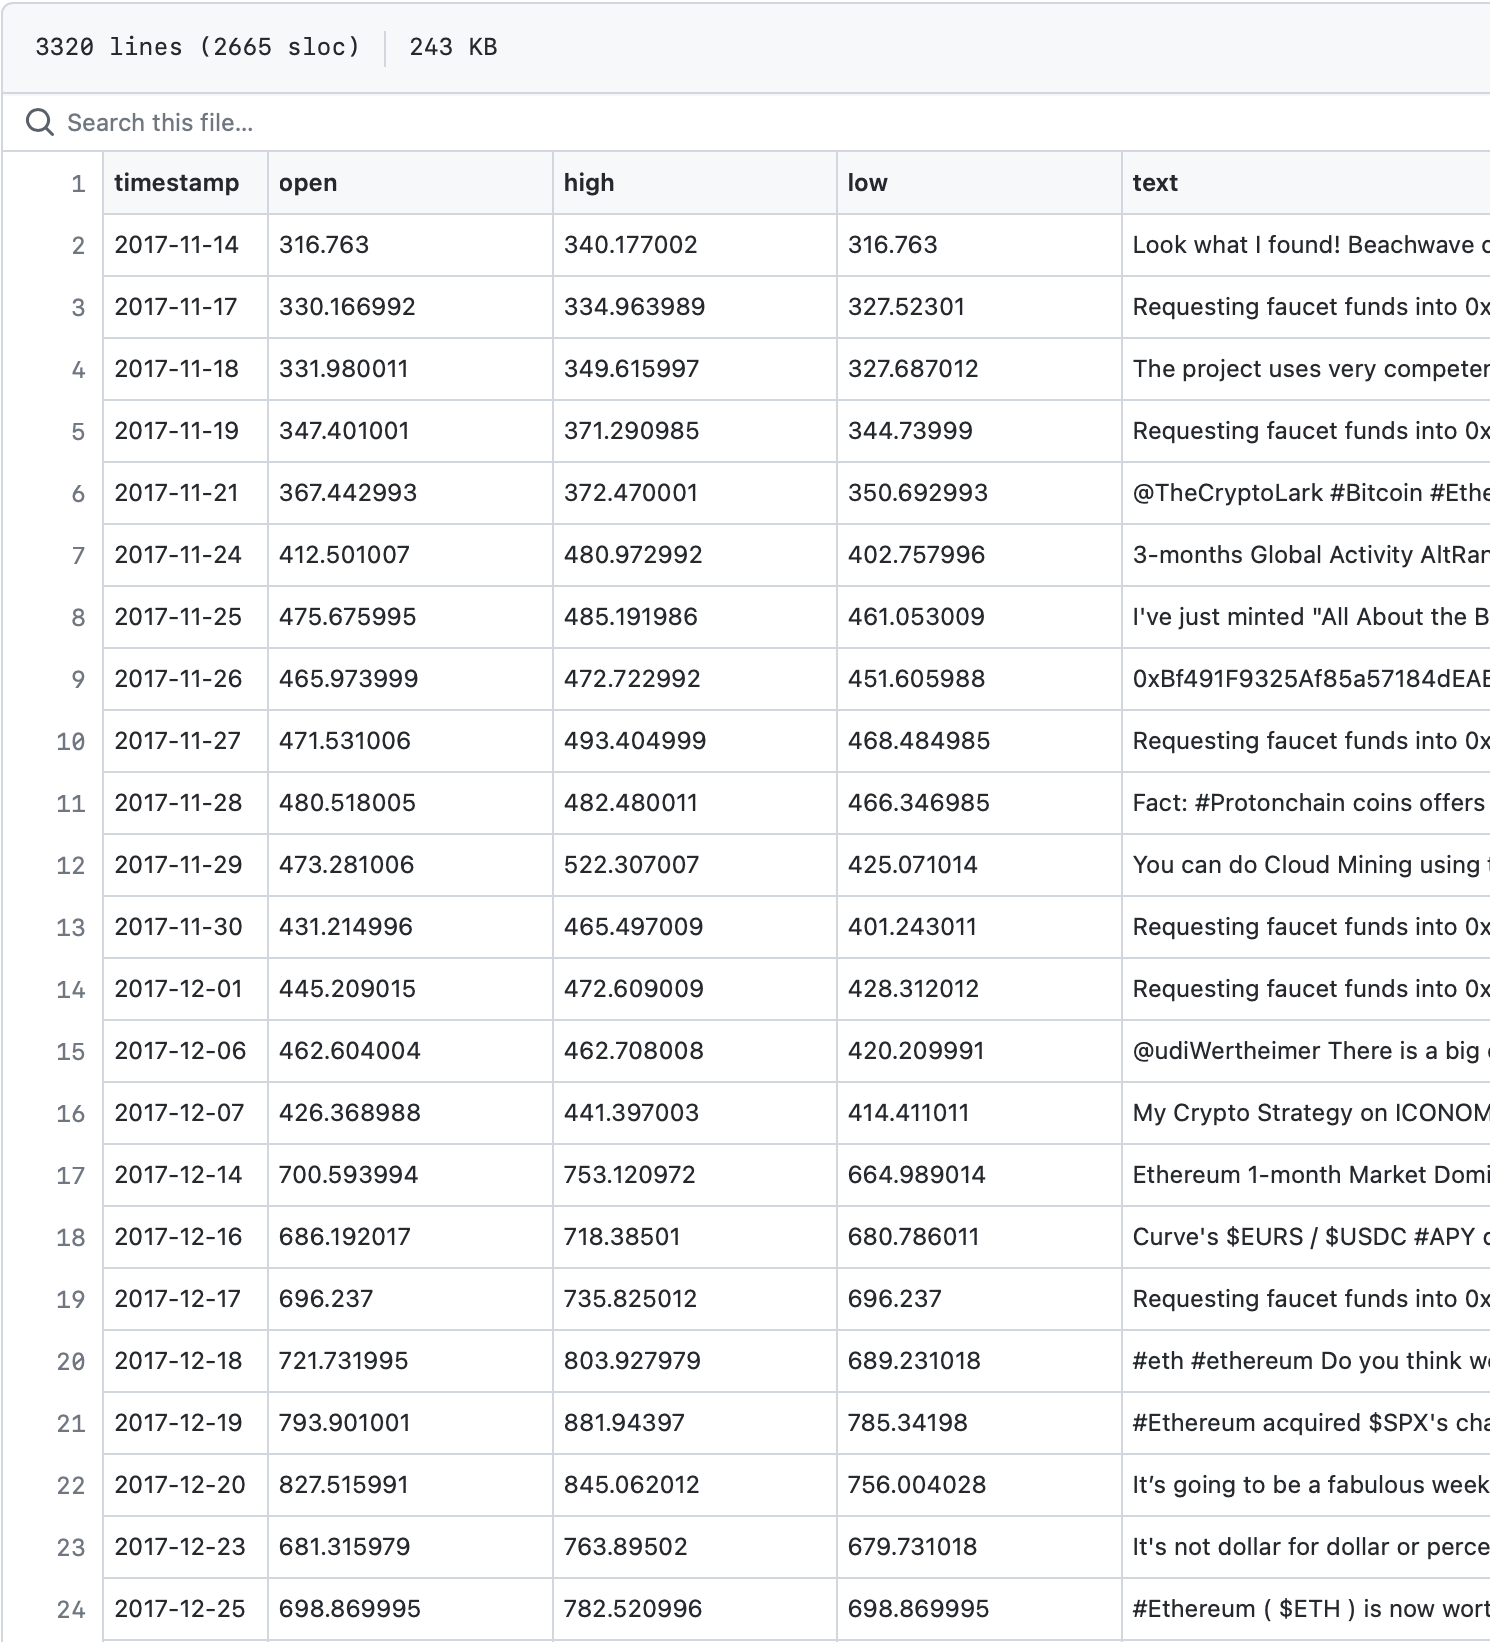
\includegraphics[scale=0.30]{images/ethereum-sample-cleaned-dataset.png}
    \caption{
        Pictured here is a sample of the cleaned Ethereum data set, showing the kept columns: timestamp, open, high, low, and text. Note, the text column was cut short for visualization purposes.
    }
    \label{sample-cleaned-dataset}
\end{figure}


\subsection{Sentiment Analysis}

After pre-processing the data, sentiment analysis was performed. The built-out sentiment analyzer ingested these output files from the cleaning step and calculated the following sentiment scores for each row of the textual news column:

\begin{itemize}
    \item subjectivity
    \item polarity
    \item compound
    \item negative
    \item neutral
    \item positive
\end{itemize}

\noindent According to \textcite{sentimentanalysis}, compound is ``the sum of positive, negative \& neutral scores which is then normalized between -1 (most extreme negative) and +1 (most extreme positive)". In other words, as \textcite{vadersentiment} put it, compound is a ``normalized, weighted composite score". Meanwhile, subjectivity, polarity, negative, neutral, and positive are measures of their exact meaning. A range of scores were computed to expand the span of quantitative analysis and capture a breadth of features.

This sentiment analysis was done using \textbf{VADER Sentiment Analysis}, the tool created by \textcite{vadersentiment}, following the YouTube tutorial \href{https://www.youtube.com/watch?v=4OlvGGAsj8I}{Stock Market Sentiment Analysis Using Python \& Machine Learning}, with refactoring added to organize the code more logically and ingest and output data in accordance with the other steps of this pipeline. I chose to use this VADER Sentiment Analysis tool for its extensive documentation and its specific tuning to sentiment expressed in social media. Further, it has been used by over 4.4 thousand GitHub users, which speaks to its ease of use and solidity \cite{vadersentiment}. Because of this tuning, I believed the tool would be well-equipped to capture the features present in the training set, which was collected across news outlets and social media sites (Twitter and Reddit).

These sentiment scores were then appended to the originally ingested data set as new columns and the previous text column was removed, as only the sentiment calculations are needed as input to the price prediction algorithm and excess columns may add unnecessary computational slowdown. The resulting data set was outputted as a new file, maintaining the input data sets intact. This outputted file was the input to the LSTM price prediction model.

\begin{figure}
    \centering
    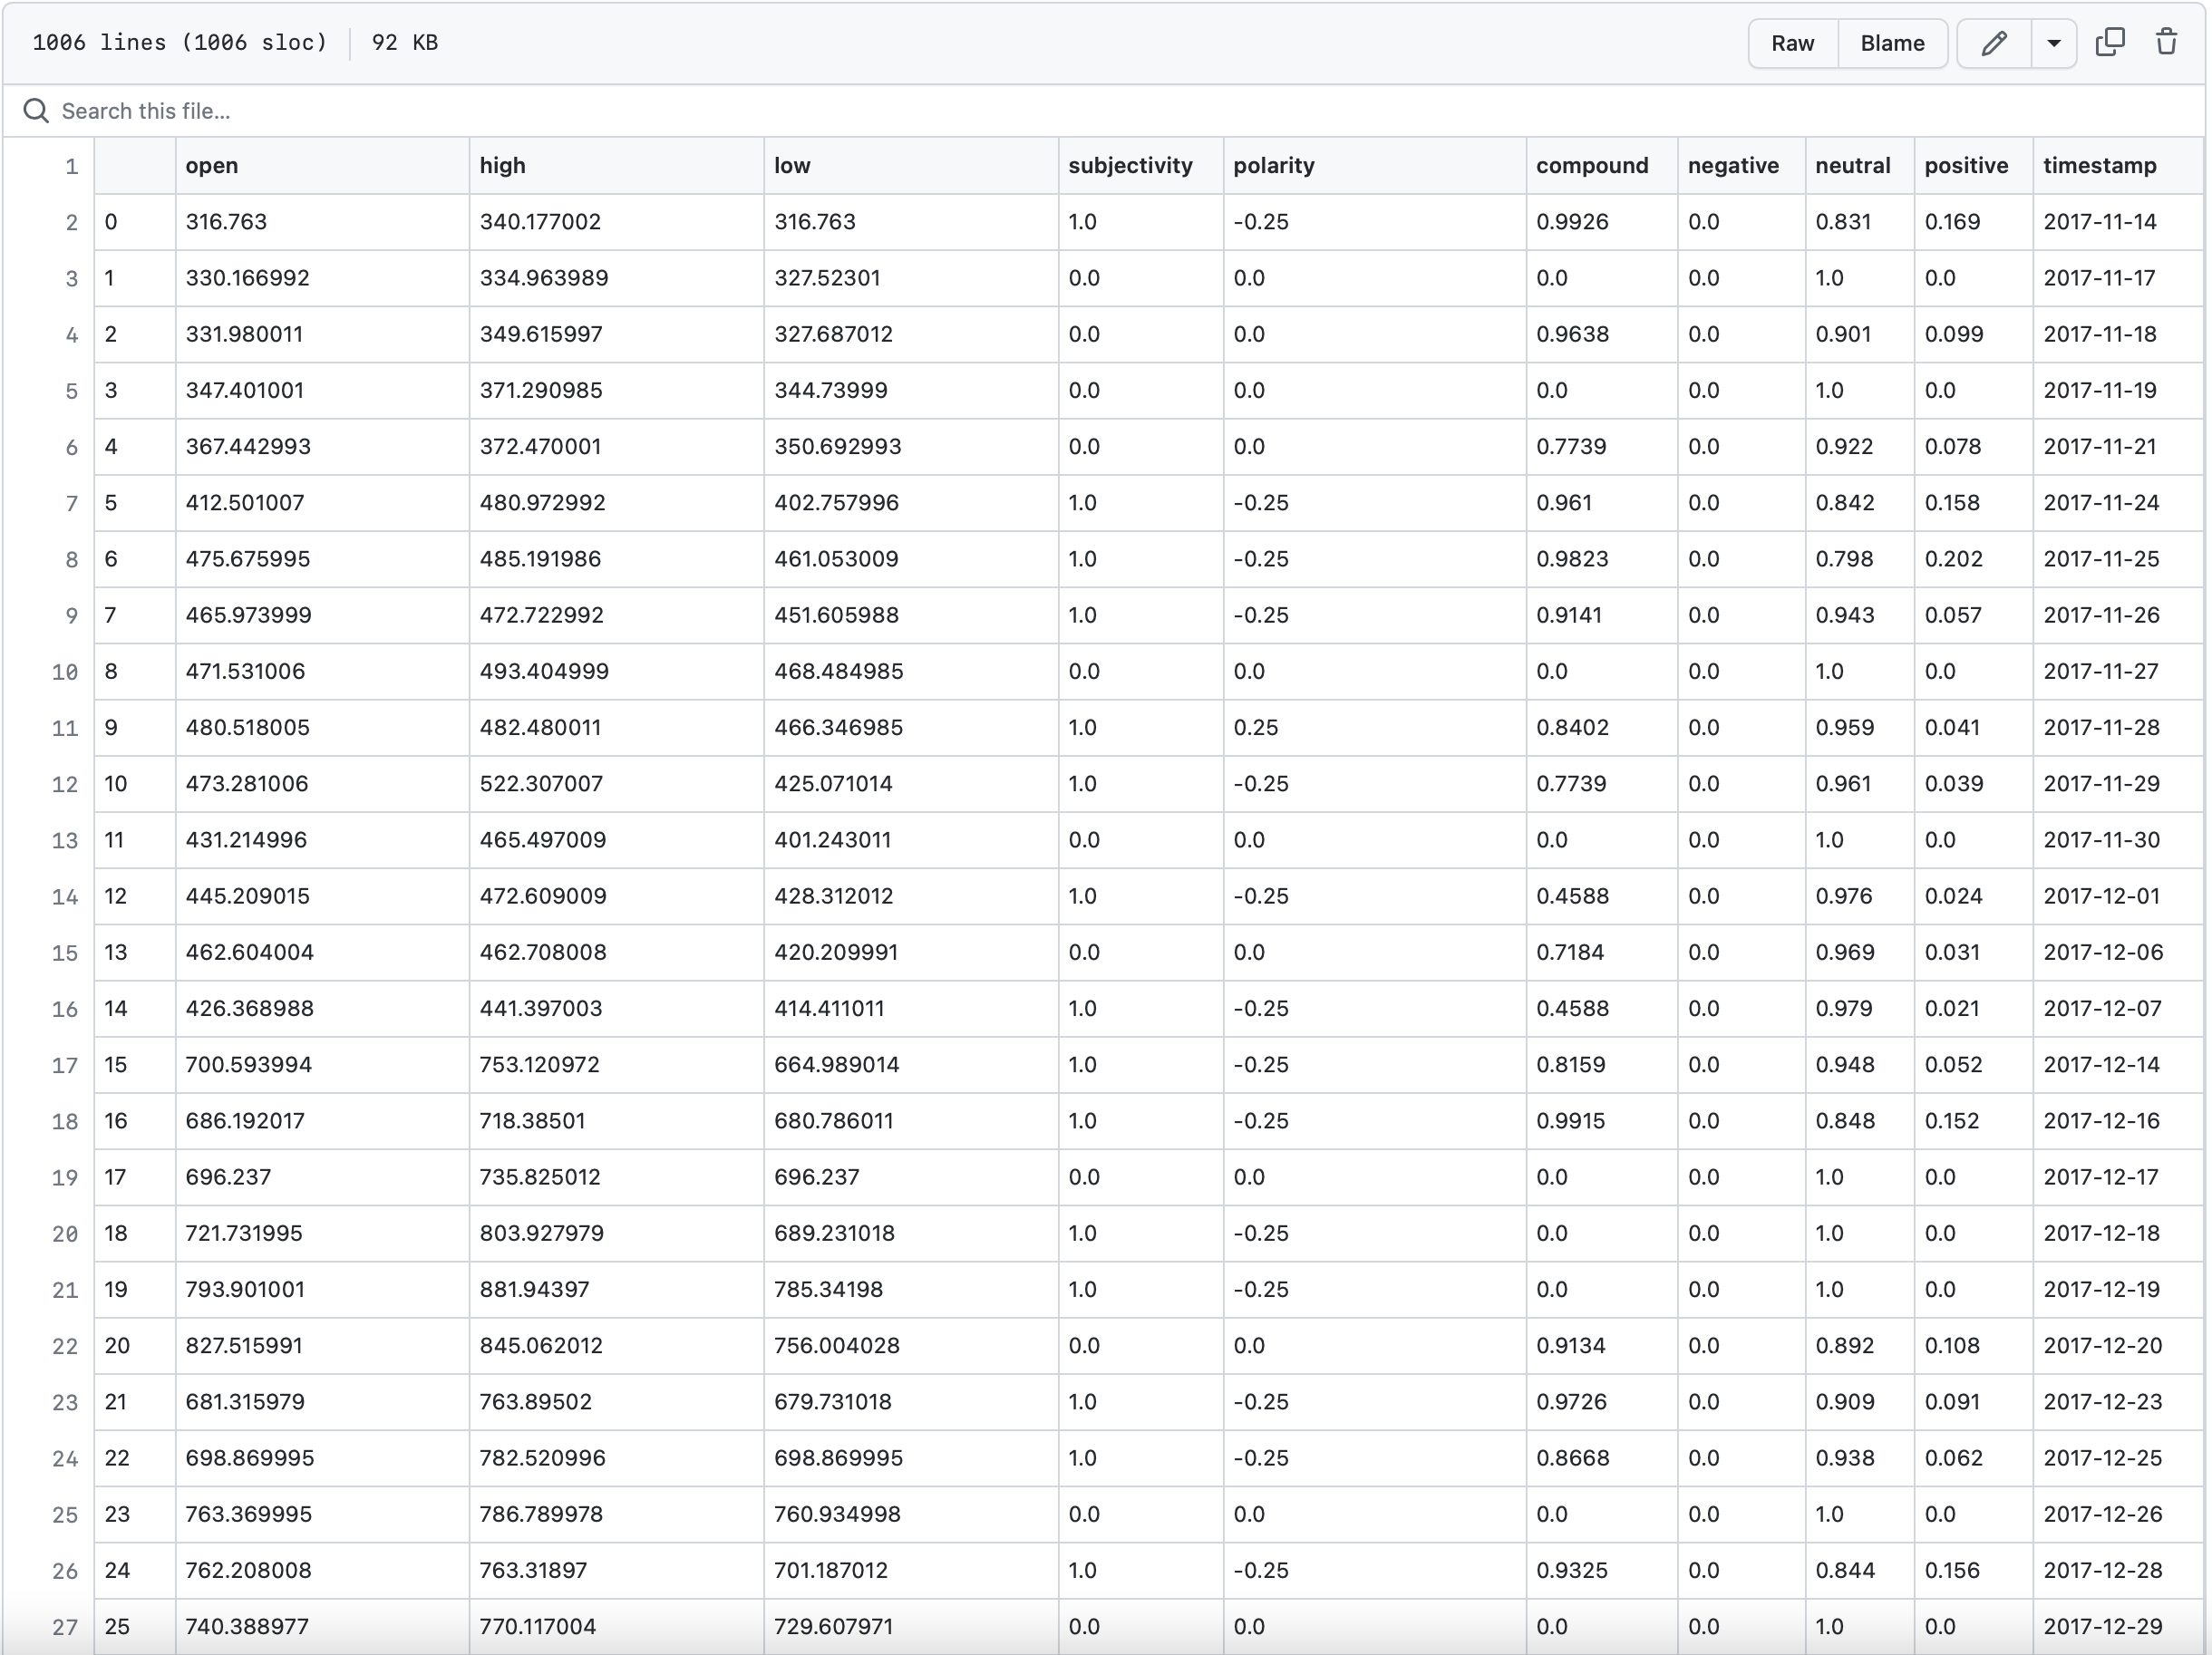
\includegraphics[scale=0.18]{images/ethereum-sample-sentiment-analysis-output.png}
    \caption{
        Pictured here is a sample of the output of the sentiment analysis process for Ethereum with the kept columns: timestamp, open, high, low, subjectivity, polarity, compound, negative, neutral, positive, timestamp.
    }
    \label{sample-sentiment-dataset}
\end{figure}

\subsection{LSTM Price Predictions}

A long short-term neural network (LSTM) was used to perform price predictions for the cryptocurrencies with available data. As mentioned in the sections \ref{RNN-LSTMs} and \ref{longshorttermneuralnetworks}, LSTMs are a prime choice for time-series price predictions because they factor for both long-term and short-term trends in their analysis while concurrently solving the vanishing gradient problem and long-term dependence issues to outperform tradition recurrent neural networks (RNNs) in such time-series problems. Since LSTMs typically outperform RNNs in time-series predictions, it was clear to proceed with these neural networks for addressing cryptocurrency price predictions.

There are many flavors of LSTMs. Since I wanted this LSTM to consider an array of sentiment scores in addition to historical prices for this time-series problem, I needed to use an LSTM that accepts multiple features (aka a multivariate LSTM). For this prime multivariate LSTM model, I followed the tutorial \href{https://charlieoneill.medium.com/predicting-the-price-of-bitcoin-with-multivariate-pytorch-lstms-695bc294130}{Predicting the price of Bitcoin with multivariate PyTorch LSTMs}. In this tutorial, the author used the metrics ``high", ``low", and ``close", and ``volume" grouped by date as the input features to predict future ``open" prices. I kept my output feature the ``open" price as well. Similarly, I used an Adam optimizer and the mean squared error for the loss, which measures how well neural network models the training and is aimed to be minimized \cite{lossfunctions}. The mean squared error is a measure of the difference between the actual and predicted values, or, rather, prices in this case -- we seek to minimize this value so that our predicted price are as close as possible to the actual prices (see \nameref{price-prediction-evaluation} for further explanation). However, since my input features were different, I had to refactor the code to accept my additional and differing input features. I also had to refactor the code to accommodate shorter input and output series. Additionally, I refactored the code for clarity, building out a class from this base code, grouping snippets into logical functions, and commenting all the code with complete method stubs.


\subsection{Index Fund Rebalancing Algorithm}

The index fund re-balancing algorithm used in the available pipeline was a slight variation on that created in \textcite{algorithmictrading}, which revolves through a preset number of stocks based on their performance across a fixed period of time. The algorithm implemented here was nearly identical, with variations to support the shorter re-balancing period allotted by the future price predictions. This algorithm, however, was implemented to be used in comparison against a novel trading algorithm, which is still being hashed and included in theory for future work. This algorithm (currently in production) aims to utilize the predicted prices and their respective accuracies, depending on the coin, in conjunction with the predicted values and our aim to maximize profits in the re-balancing business logic, at which point the varied implementation of the algorithm from \textcite{algorithmictrading} can be used solely for evaluation purposes.


\subsection{End-to-End Pipeline}

To fully realize my project's goals, I built out an end-to-end pipeline. This pipeline follows:

\begin{enumerate}
    \item For each coin:

    \begin{enumerate}
        \item Collect its price across the past 30 days.
        \item Collect related news from the past 30 days.
        \item Combine and format the price and news data into a cohesive data set compatible for input to the sentiment analyzer.
        \item Pass the formatted combined data set to the sentiment analyzer.
        \item Perform sentiment analysis and save the output.
        \item Pass the output of the sentiment analysis process to the trained LSTM model for price predictions.
        \item Retrieve predicted prices and save the predicted prices.
    \end{enumerate}

    \item Combine and format the individual coins' predicted prices into a cohesive data set compatible for input to the re-balancing algorithm.
    \item Re-balance the index fund according to these predicted prices.
\end{enumerate}

\paragraph{Collecting Previous Prices}

To collect each coin's price from across the past 30 days, I used the \textbf{yfinance} library \cite{yfinance}, specifying the end date for downloading the prices as today and the start date as today minus 30 days (the day 30 days ago). The dataframe returned from the yfinance query is altered to change the column headers to follow the standard naming convention employed across this project. This information is saved for each coin as a separate csv file.

\paragraph{Collecting Corresponding Related News}

Related news for the past 30 days is collected for each coin using the \textbf{News API}. The API is used to query news sources for all headlines containing the coin's name in them. For each coin this news file is saved as a separate csv file.

\paragraph{Combining Price and News Data}

The price and news data are then combined, with the textual news column grouped by timestamp so there is only one row per date. If no news was found for a given date, the text ``neutral" is stored as the value corresponding to the text column for that row. This is saved as a single csv file.

\paragraph{Sentiment Analysis}

The sentiment analyzer reads in the the clean, combined price and news data frame and performs sentiment analysis on it. The result of this sentiment analysis is saved as a new, separate csv file for each coin.

\paragraph{LSTM Price Predictions}

The LSTM model is called on the sentiment analysis output file to predict future prices for each coin 15 days into the future. The predicted prices are saved as a new, separate csv file for each coin.

\paragraph{Combining Predicted Prices}

After all the future prices have been predicted for each coin, the results are combined into a cohesive csv file and formatted according to the pattern required for the index fund re-balancing algorithm. This is saved as a single, cohesive csv file.

\paragraph{Rebalancing the Index Fund}

With the cohesive price predictions csv file, the re-balancing algorithm re-balances the index fund. The output of this is displayed to the user.

\subsubsection{Streamlit App}

For proof of concept, I used \textbf{streamlit} \cite{streamlit}, an open-source app framework, to build out a very simple UI from where this end-to-end process can be kicked-off. The home page for this simple UI is pictured in Figure \ref{streamlitapp}.

\begin{figure}
    \centering
    \tcbox[sharp corners, boxsep=5mm, boxrule=1mm, 
            colframe=black, colback=white]
            {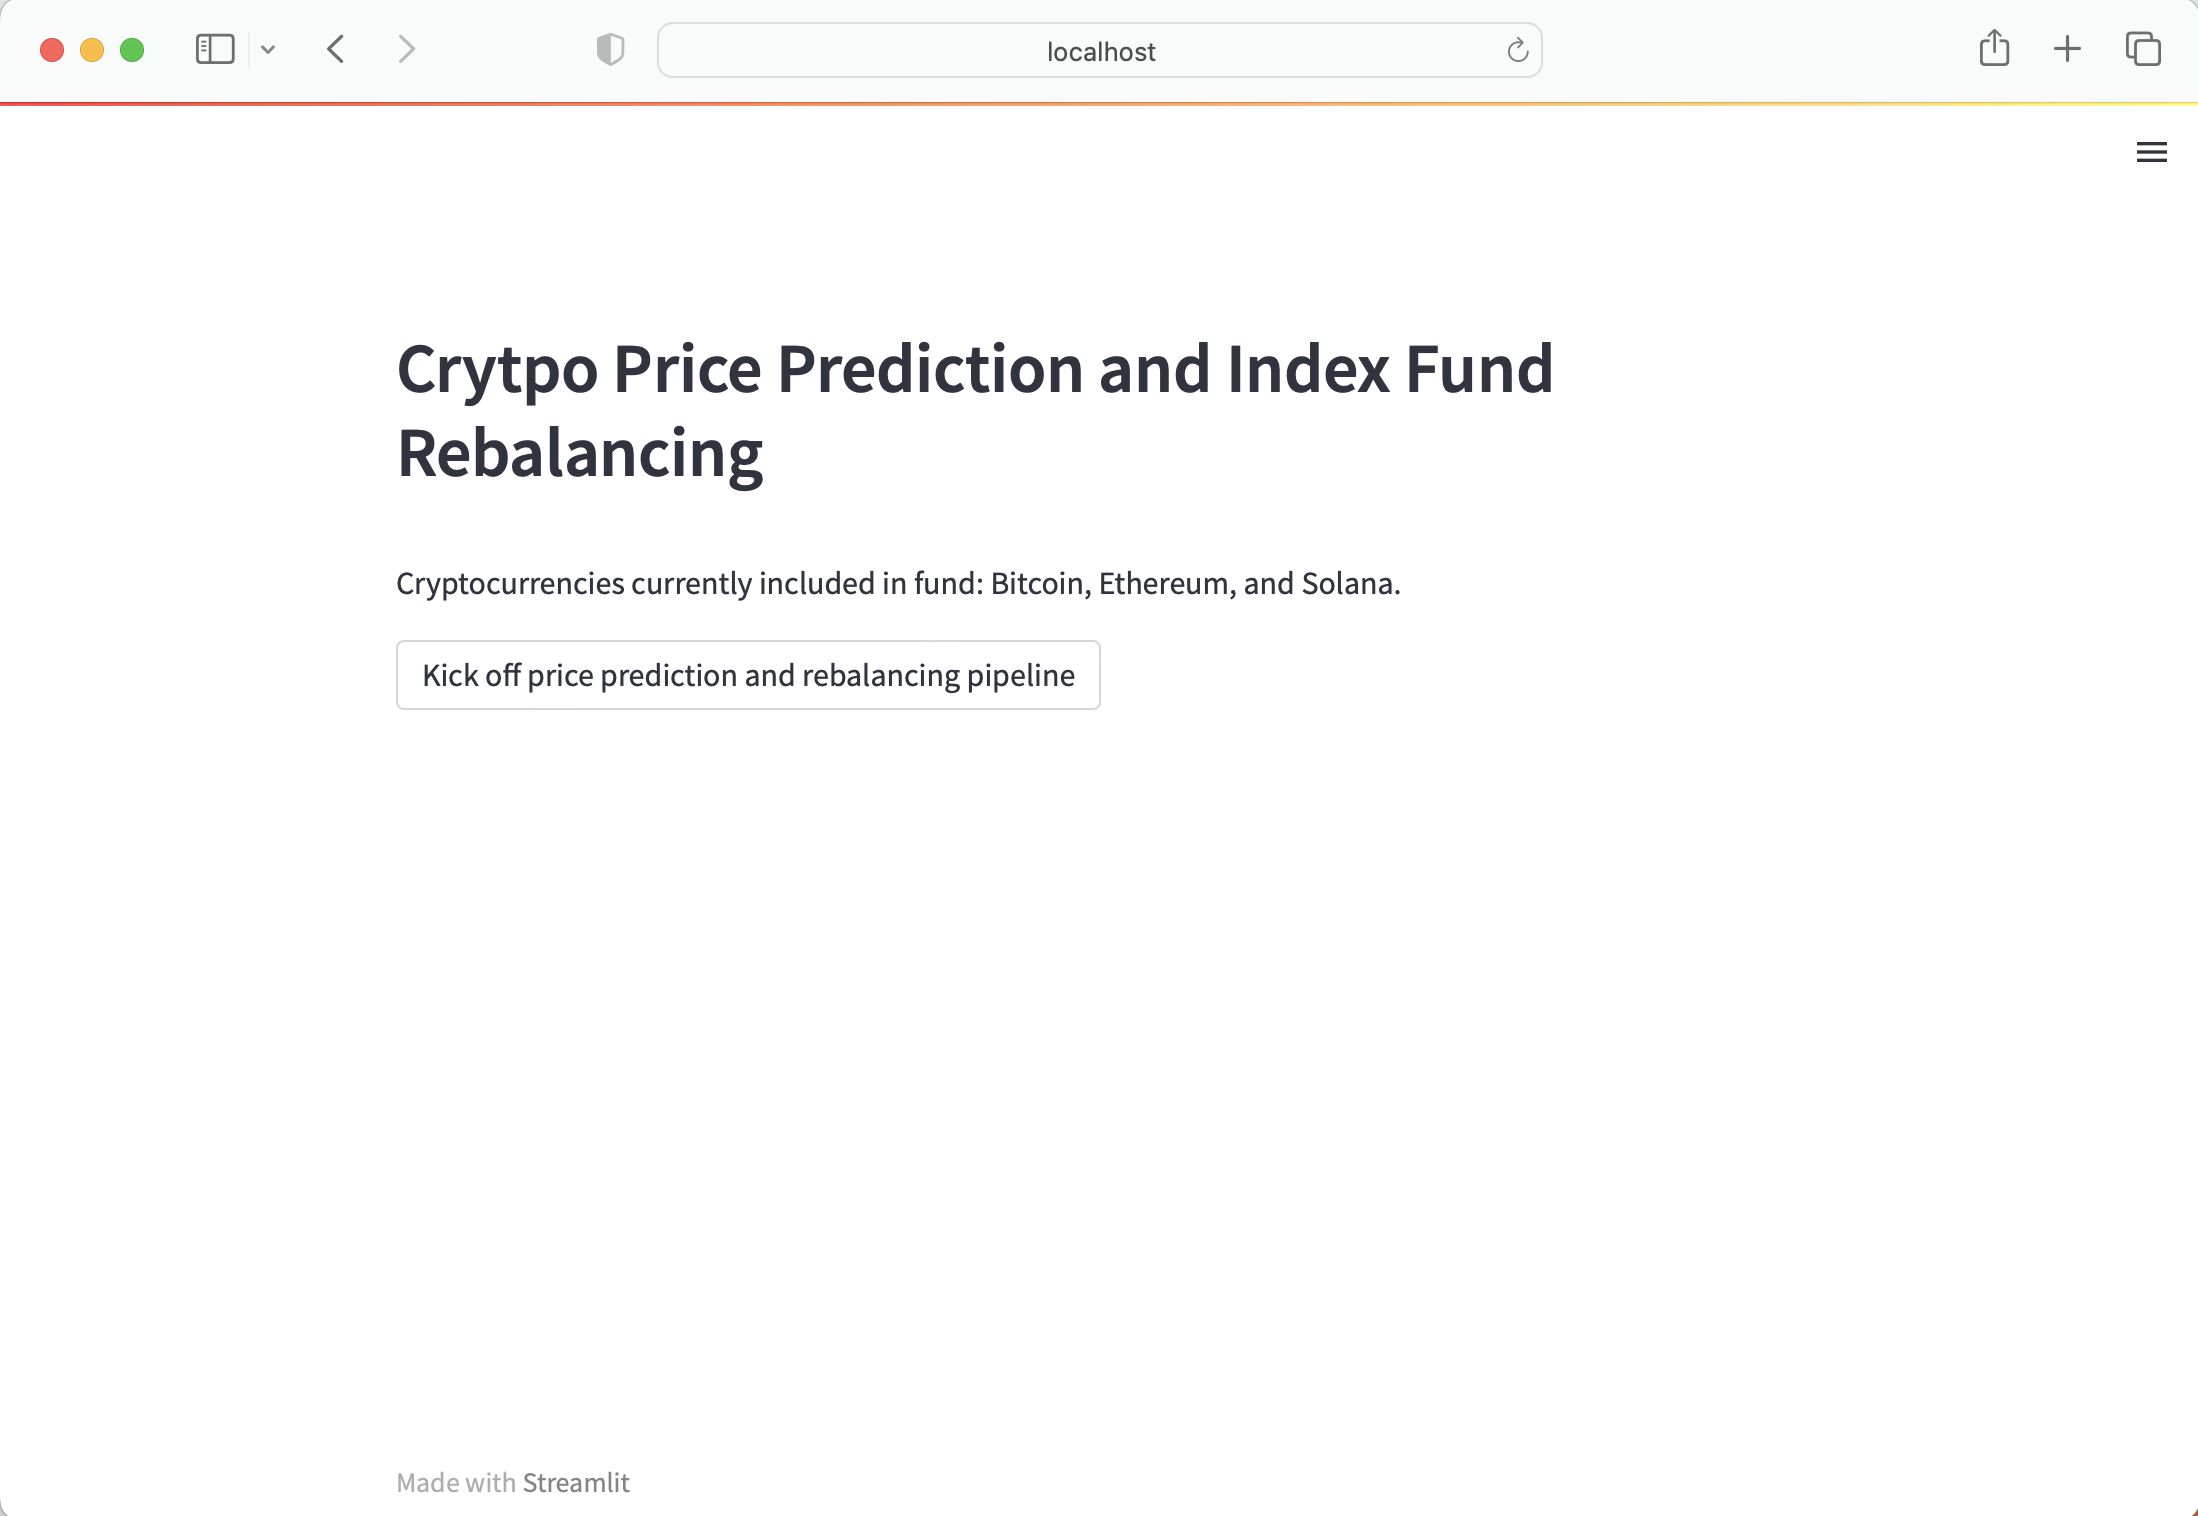
\includegraphics[scale=0.16]{images/streamlit_app.png}}
    \caption{
        Streamlit app home page for this project's end-to-end pipeline.
    }
    \label{streamlitapp}
\end{figure}


\section{Evaluation Metrics} \label{evaluationmetrics}

Were the rebalancing algorithm to work based on bad predictions, regardless of its ingenuity and logic, we would expect its results be poor. Similarly, if the price predictions are highly accurate but the rebalancing algorithm is defective, we may see poor overall results. Essentially, it may be impossible to discern where fault lies in poor results unless we evaluate these two components separately. As such, the evaluation of this project was split into two general categories: evaluation of the price predictions and evaluation of the rebalancing algorithm.

\subsection{Price-Prediction Evaluation} \label{price-prediction-evaluation}

To evaluate the multivariate LSTM model, I took two approaches:

\begin{enumerate}
    \item To evaluate the sanity of the tutorial model's logic itself, I built out adjacent models.
    \item To evaluate whether the sentiment input data affected the accuracy of the price predictions, I compared the sentiment data sets to data sets with constant sentiment scores.
\end{enumerate}

To evaluate a model, Data Scientists typically split their data set into two parts: a training set and a testing set. The training set is used to train the model, while the testing set is used to evaluate the model's performance. The split between testing and training sets varies, but it was broadly kept between 70\% to 95\% training and 5\% to 30\% testing of the original data set for this project -- in this project, the train/test split varied from coin to coin and model to model based on the amount of available data and the performance metrics from varying this split.

Using this testing data, I compared predicted results (from using the testing set's input data) against the corresponding actual prices (the testing set's output data). For machine learning models outputting binary decisions, evaluation typically consists of calculating a set of metrics such as precision and recall. In this case, the model's output is not a binary decision but a discrete value instead. Achieving perfect accuracy in the predicted prices is likely impossible, but we only need to capture the general features and trends of the price movements to have good results. So, we must measure the performance of these models with other means. I chose to measure the relative accuracy of each model by calculating the mean squared error (mse), given by

\begin{equation}
    \text{MSE} = \frac{1}{n} \sum_{i=1}^{n} (Y_i - \hat{Y}_i)^2
\end{equation}

\noindent where $n$ is the number of data points, $Y_i$ are the observed values and $\hat{Y}_i$ are the predicted values \cite{mseWikipedia}. In our case, the number of data points $n$ are the number of data points in the test set, $Y_i$ are the actual prices, and $\hat{Y}_i$ are the model's corresponding predicted prices. The mean squared error looks at the average difference between the actual prices and the predicted prices, giving a sound measurement for calculating performance. With this metric of performance, we seek to minimize the mean squared error -- a smaller mean squared error value corresponds to better predictions.

\subsubsection{Adjacent Models}

The adjacent models for the first point of comparison were:

\begin{itemize}
    \item a price-based LSTM model built with TensorFlow;
    \item a multivariate sentiment and price-based model with different logic built with TensorFlow; and
    \item a sentiment and price-based Linear Discriminant Analysis model.
\end{itemize}

\noindent These models were built to evaluate the soundness of the code for the sentiment and priced-based multivariate PyTorch LSTM based off the tutorial model. The price-based LSTM model built with TensorFlow was made to compare a TensorFlow model to a PyTorch model and to see if the sentiment inputs added much to the overall prediction accuracy. This was by far the most accurate model next to the prime model. The multivariate sentiment and price-based model built with different logic using TensorFlow was used to compare the prime model against a sample multivariate model to evaluate the logic of the code with a rather 1:1 comparison. The sentiment and price-based Linear Discriminant Analysis model was used to compare a non-LSTM model to an LSTM model to constrain whether the LSTM model was a sound choice.

The evaluation against these models generally employed the use of mean squared error as a means for measuring accuracy. The Linear Discriminant Analysis model was excepted from using the mean squared error method of evaluation since it outputs 0/1 values signifying only a predicted decrease/increase in price (0 = decrease, 1 = increase) -- we cannot compare decreases/increases in price to actual price data points. Instead, for this model, I followed the typical evaluation for binary models and used the metrics: precision, recall, f1-score, support, accuracy, macro average, and weighted average. According to \textcite{precisionandrecall}, precision is a measure of the ``proportion of positive identifications [that are] actually correct" and recall is a measure of the ``proportion of actual positives... identified correctly". Similarly, f1-score is a value that combines precision and accuracy to give a composite score.

\subsubsection{Constant Sentiment}

To evaluate whether the sentiment data had any impact on the accuracy of the predicted prices, for each coin I took the cleaned data sets outputted from the sentiment analyzer and converted all the sentiment scores to the value `1'. I then compared the prime model's performance after being trained on the actual sentiment files versus these constant sentiment files to see if the sentiment scores impacted the accuracy of the predicted prices.

\subsection{Index Fund Rebalancing Evaluation}

To evaluate the index fund, I took 15 days worth of past actual prices for the cryptocurrencies in the Bitwise 10 Crypto Index Units Beneficial Interest (BITW) fund and treated them as ``predicted future prices". This was done to eliminate the price predictions affecting the perceived validity of the re-balancing algorithms and, instead, evaluate the re-balancing algorithms assuming the price predictions were entirely accurate. Essentially, I evaluated the re-balancing algorithm under the assumption that the predicted prices inputted are entirely correct. I compared the temporary index fund's returns, created by \textcite{algorithmictrading}, to the returns produced by BITW, using the metrics of compound annual growth (CAGR), volatility, the sharpe ratio, and the maximum drawdown with the implementations by \textcite{algorithmictrading}. Once the pending index fund re-balancing algorithm is fully finished, I plan to evaluate its performance against both the simple re-balancing algorithm implemented here and the BITW fund results using the same evaluation metrics.

\section{Results and Discussion} \label{resultsanddiscussion}

The section follows the split between the evaluation of the predicted prices and re-balancing algorithm introduced under \nameref{evaluationmetrics}, with the results of each initially discussed separately. The joint results are then viewed in the context of this project's overall goals.

\subsection{Predicted Prices}

The predicted prices were evaluated using the two methods above: alternative models and constant sentiment. The results of comparisons of the prime model against alternative models are first discussed.

\subsubsection{Alternative Models Comparison}

\paragraph{Price-Based TensorFlow LSTM Comparison}

The prime model was compared against a price-based LSTM model built with TensorFlow based on the tutorial by \textcite{PriceLSTMModel}. This TensorFlow model, which inputted historical prices alone in its prediction of future prices, was the most accurate model next to the prime model. The outputs of this can be viewed under the project folder located under \textit{src.models.outputs.graphs} by viewing the related files:

\begin{itemize}
    \item PriceLSTMModel\_comparison\_bitcoin.png
    \item PriceLSTMModel\_comparison\_ethereum.png
    \item PriceLSTMModel\_comparison\_solana.png
\end{itemize}

Note, this model had a higher input length, which increased the accuracy of the price predictions. With an increased input length, the prime model's accuracy also increased. This model did not prove that the business logic driving the prime model was necessarily superior, but the comparison did suggest the respective logic driving each model is comparable.

\paragraph{Multivariate Sentiment and Price-Based Differing Logic TensorFlow Comparison}

The multivariate sentiment and price-based TensorFlow LSTM model (based on differing logic from \textcite{SampleSentimentLSTMModel}) was fairly unsuccessful; the trained model failed to capture the trends of price prediction. Comparing this model to the prime model concluded the prime model to be considerably more successful. As this was a rather 1:1 comparison seeing as they had the same input data, this further affirmed the validity of the logic behind this prime model's code. The outputs of this can be viewed under the project folder located under \textit{src.models.outputs.graphs} by viewing the related files:

\begin{itemize}
    \item SentimentLSTMModel\_comparison\_bitcoin.png
    \item SentimentLSTMModel\_comparison\_ethereum.png
    \item SentimentLSTMModel\_comparison\_solana.png
\end{itemize}

\paragraph{Sentiment and Price-Based Linear Discriminant Analysis Comparison}

The results obtained from analyzing the Linear Discriminant Analysis, based off the model developed in this tutorial \textcite{SampleSentimentModel}, performance according with the outlined evaluation metrics were very poor. For Bitcoin, which had the largest data set by far, spanning the course of nearly seven years, the results were still fairly deplorable. These results can be pictured in the table \nameref{linearDiscriminantResultsBitcoin}.

\begin{tabular}{ |p{1.25cm}||p{1.15cm}|p{1cm}|p{1cm}|p{1cm}|  }
 \hline
 \multicolumn{5}{|c|}{Linear Discriminant Results for Bitcoin} \\
 \hline
  & precision & recall & f-score & support \\
 \hline
 0 & 0.38 & 0.08 & 0.13 & 211 \\
 1 & 0.50 & 0.88 & 0.64 & 221 \\
 \hline
 accuracy & & & 0.49 & 432 \\
 macro avg & 0.44 & 0.48 & 0.38 & 432 \\
 weighted avg & 0.44 & 0.49 & 0.39 & 432 \\
 \hline
\end{tabular}
\label{linearDiscriminantResultsBitcoin}

The relative high accuracy of the prime LSTM model compared with this Linear Discriminant Analysis model promoted the choice to use an LSTM, affirming the approach backing price-prediction in this project.

\subsubsection{Constant Sentiment Comparison}

The comparison between the predicted prices outputted from the same prime model trained on the actual sentiment input data versus the constant sentiment input data showed that the model trained on the sentiment data was more accurate. The outputs of this constant sentiment evaluation can be viewed by comparing the project files located at \textit{src.evaluation.outputs.graphs}, representing the constant sentiment outputs, with those under \textit{src.models.outputs.graphs} beginning with \textit{SentimentPriceLSTMModel}, which represent the outputs of the prime model.

\begin{figure}
    \centering
    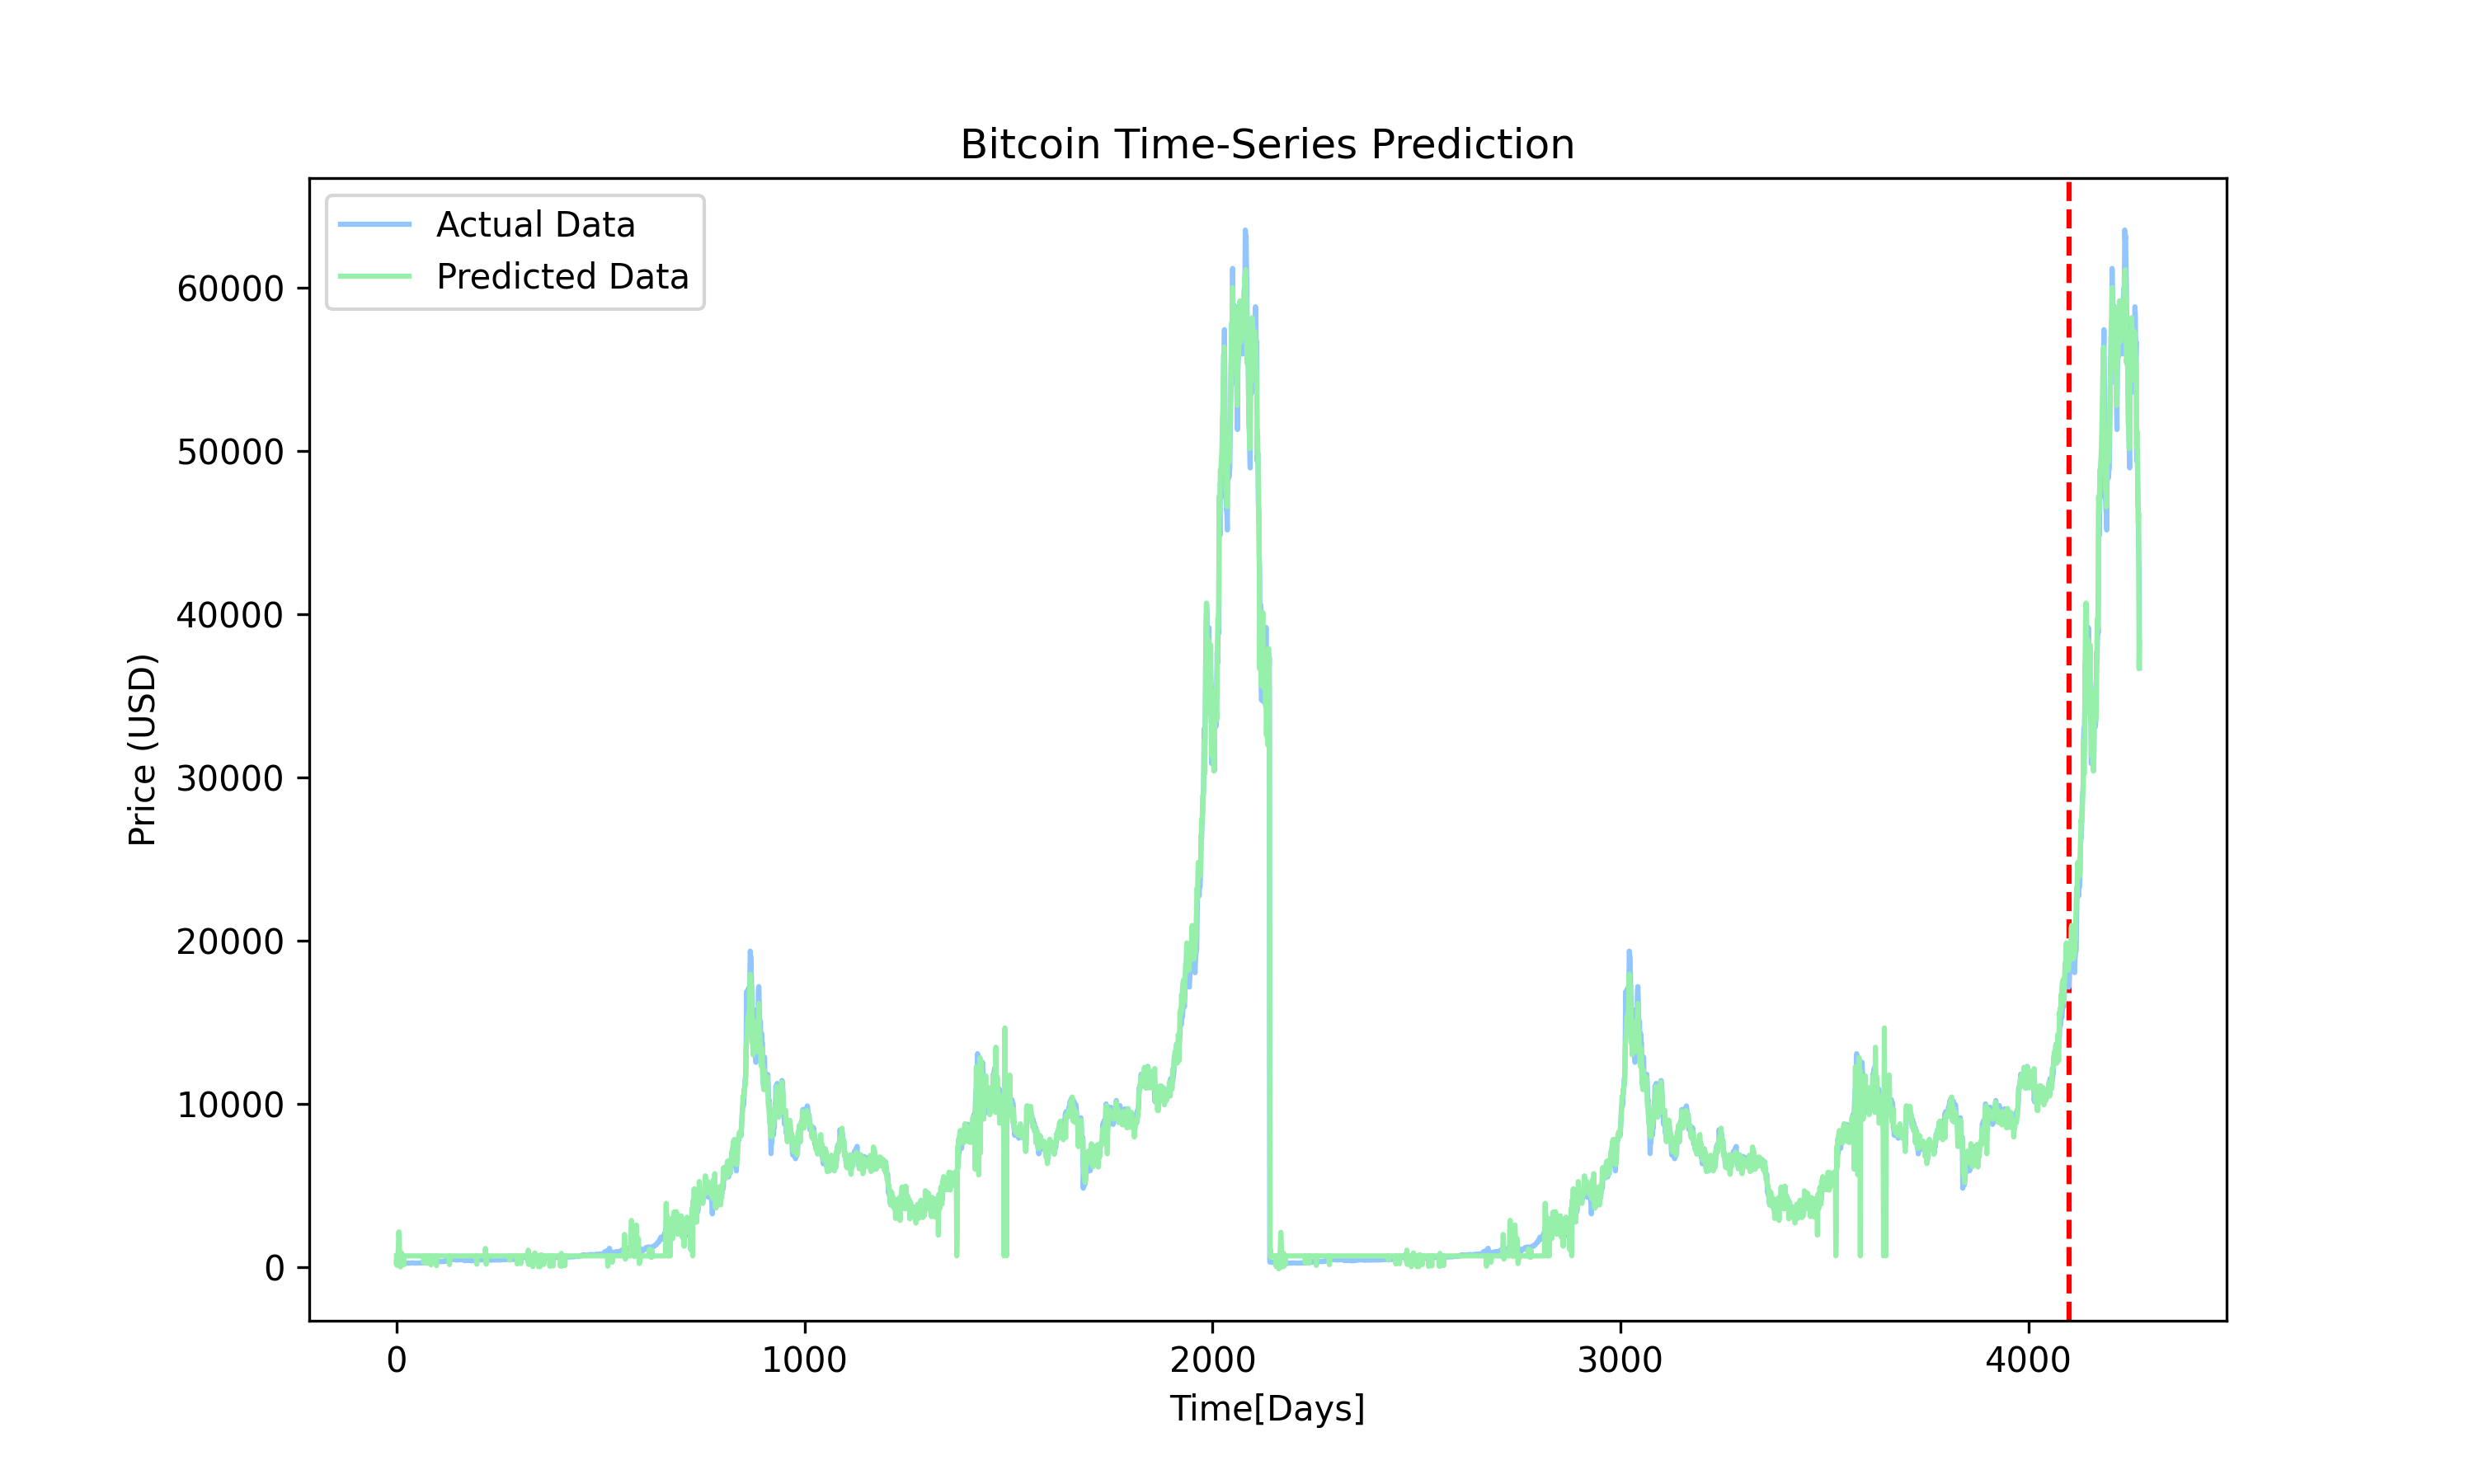
\includegraphics[scale=0.35]{images/SentimentPriceLSTMModel_whole_plot_bitcoin.png}
    \caption{
        This image shows the prime model's time-series predictions against the actual prices from the same time.
    }
    \label{sentiment-price-lstm-whole-plot}
\end{figure}

The improved accuracy in using a model trained on sentiment data proves that the sentiment data is useful in predicting prices. This result suggests that sentiment is, indeed, a good indicator for cryptocurrency prices.

\subsection{Rebalancing Algorithm}

The final rebalancing algorithm has yet to be fully implemented, so the evaluation compared the varied implementation by \textcite{algorithmictrading} against the performance of the BITW fund. Surprisingly, the algorithmic trading algorithm outperformed the BITW fund on the same stocks, suggesting this re-balancing algorithm, though simple, has promising results.

\begin{figure}
    \centering
    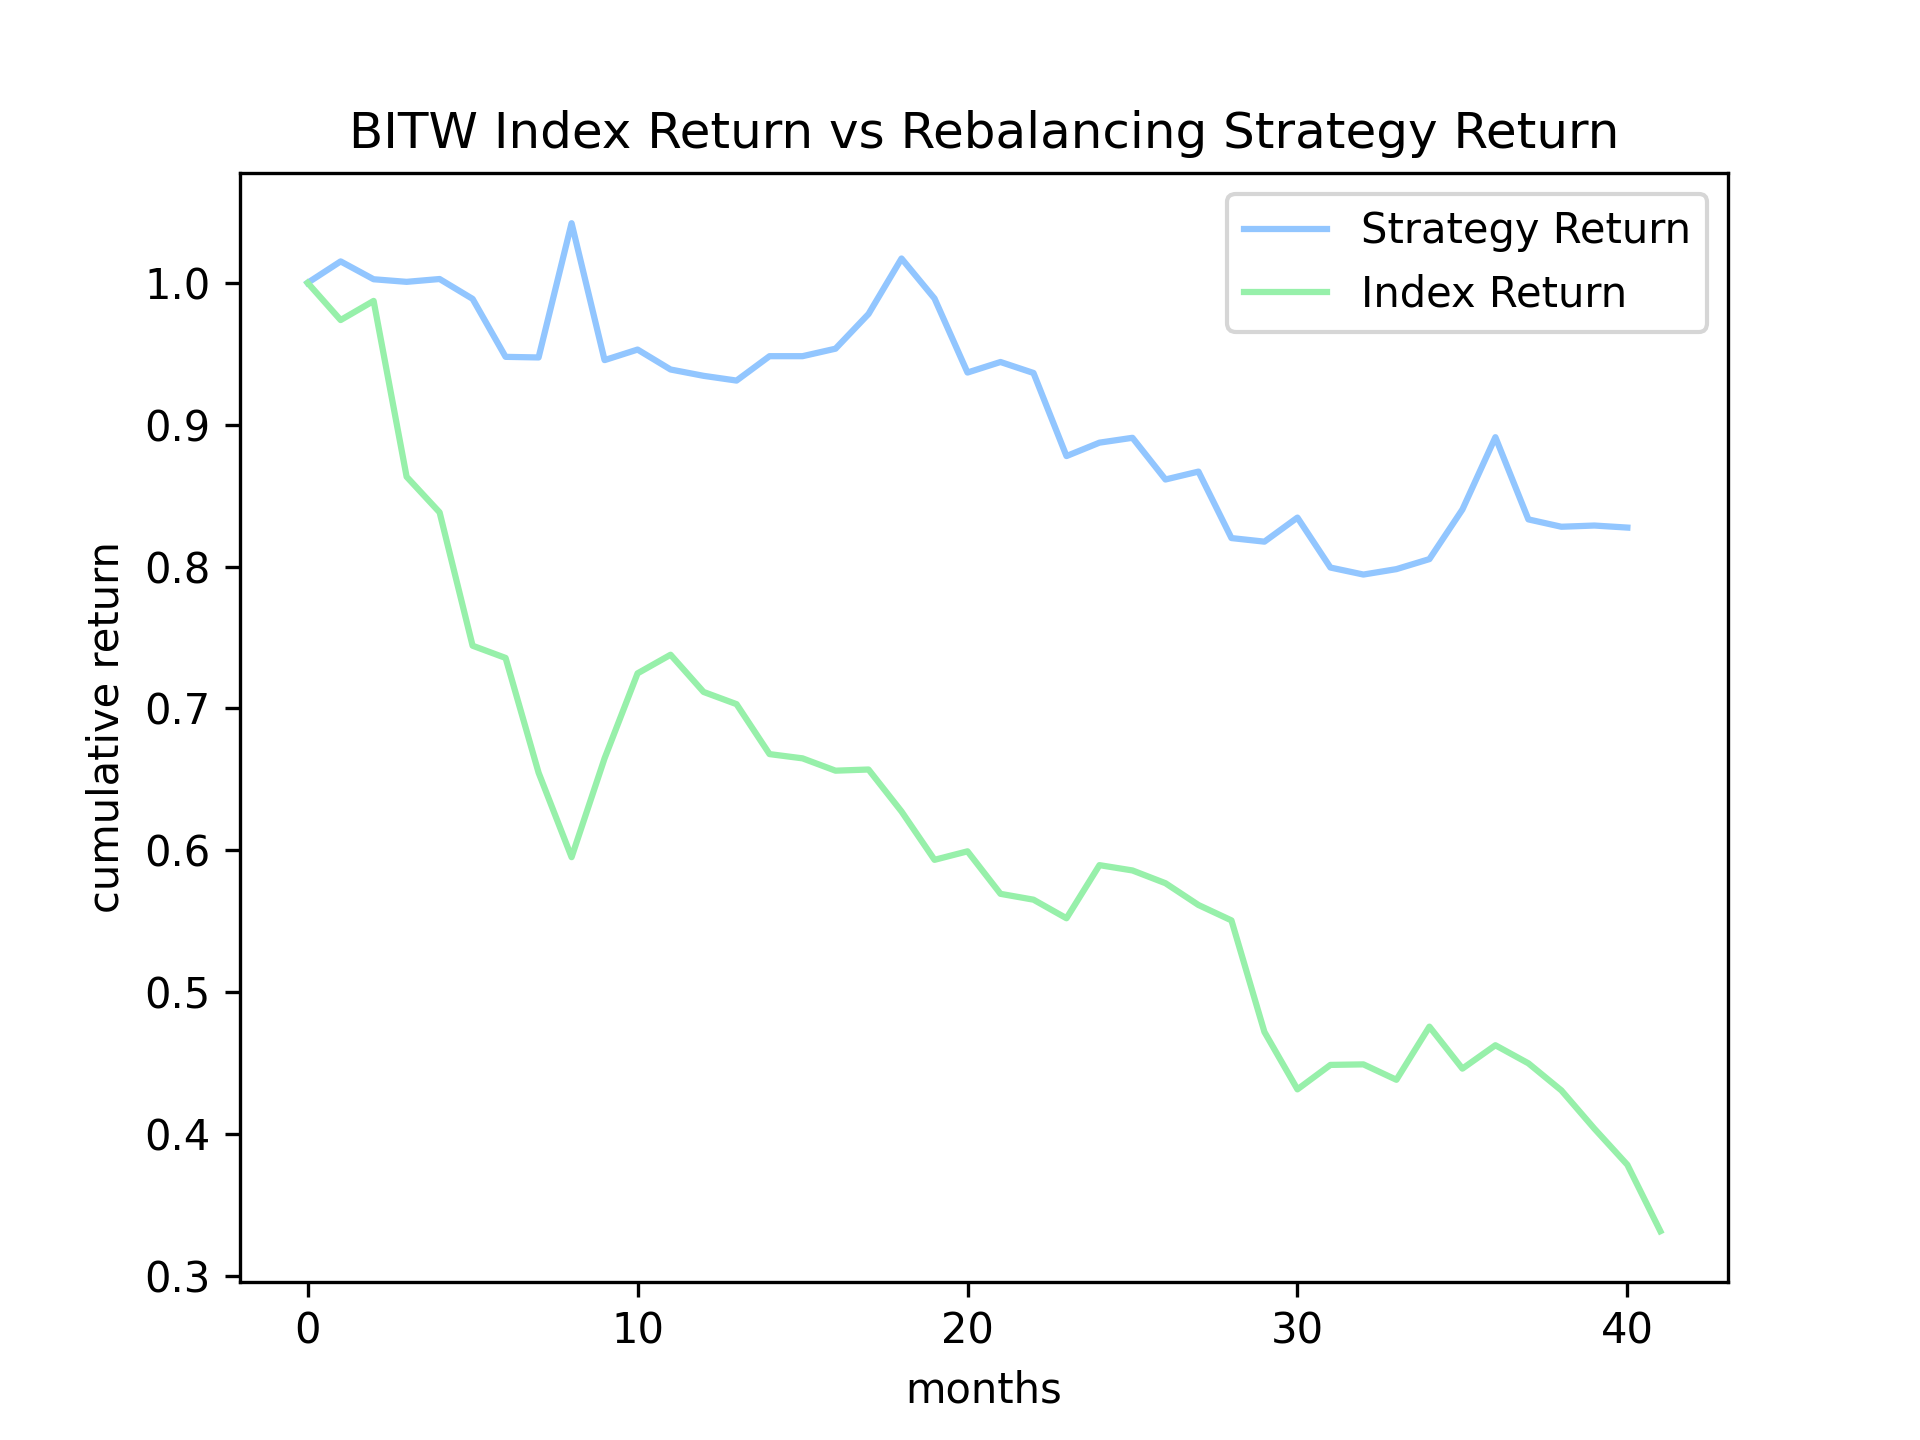
\includegraphics[scale=0.50]{images/index_return_vs_rebalancing_strategy.png}
    \caption{
        This image shows the algorithmic re-balancing algorithm's returns compared to the returns given by the BITW fund on the same coins during the same period. This comparison was developed by \textcite{algorithmictrading}.
    }
    \label{re-balancing-algorithm-results}
\end{figure}

\subsection{Collective Results}

Overall, the price predictions generated by the prime model were fairly accurate. Despite the predictions never being exact, they captured the general trend of price movement. The results of this project are promising. This project was made as a proof of concept, succeeding in its goal to build a fully-functional end-to-end pipeline. Further, it showed promising initial results for cryptocurrency price prediction alone and in conjunction with re-balancing index funds, suggesting future versions of this work could have increased success in leveraging the volatility of these currencies and maximizing gains in investments.

\section{Ethical Considerations} \label{ethicalconsiderations}

When considering the ethical considerations of predicting cryptocurrency prices for stock trading using machine learning, we must break the question into sub-tasks. Since this project advocates for the use of cryptocurrencies, we must consider the ethics of cryptocurrencies themselves. Further, we must look into the ethics of stock trading and the investor obligations that come into play when building an index fund, especially one built with machine learning.

\subsection{Nature of Cryptocurrency}

Due to the immutability of blockchain, and, hence, cryptocurrencies, the risk of tampering by bad actors is eliminated, creating a trustworthy network. Traditionally, information storage and retrieval systems were susceptible to cyberattacks. Moreover, without transparency on behalf of the record-management company or system, record tampering would be harder to catch and verify. The open-book nature of blockchain allows for widespread verification of all transactions. Coupled with the blockchain's immutable nature, with no user nor managing power having the ability to alter or delete a transaction, blockchain technologies, and, hence, cryptocurrencies, are extremely safe from a tampering standpoint \cite{WhatIsBlockchain}. This addresses transparency on behalf of the cryptocurrency operations, but it does not cover the ethical considerations with regard to the security of such assets.

A second consideration is the instability of where cryptocurrencies are hosted. One Washington Post Article, \citetitle{TrackingStolenCrypto}, details the commonality of crypto heists. Hackers have previously hacked into cryptocurrency trading networks, getting away with massive sums. In August of 2021, Poly Network, a trading platform for popular cryptocurrencies, was hacked, with the hackers taking 
\$610 million in crypto, which they quickly converted to a ``stable coin". Luckily, the ``stable coin" Tether worked with authorities to release the holdings to the rightful owners. Nonetheless, this heist broke the belief that cryptocurrency is impossible to trace (public ledgers do not retain account holder information) \cite{TrackingStolenCrypto}. The anonymity of cryptocurrencies may be ethical, guarding the identity of its users or not, allowing for bad actors to use crypto for illicit activities, but it is certain that their online holdings make them susceptible to being stolen, further questioning the security of their nature.

Despite the secure theoretical ideas behind cryptocurrencies, their value is often in flux. Ethicists have previously questioned the ethics of cryptocurrencies themselves. Professor Tobey Karen Scharding shared her evaluation of bitcoin from an ethical perspective in an interview at Rutgers Business School:

\begin{quote}
    With bitcoin, I felt there were too many uncertainties... [The] evaluation was pretty negative because bitcoin didn't really have any way to secure its value, and so it wouldn't be able to fulfill the ethical purpose of currency on Fichte's account of stabilizing and securing these exchanges over generations. \cite{IsBitcoinEthical}
\end{quote}

Professor Scharding refers here to the Fichte account, which explains that currency should allow people to live their lives with secure access to basic goods and services and allows them to enjoy life and exchange goods with other people. By Professor Scharding's logic, cryptocurrency falls short of being an ethical currency because its often-changing value means that one day it could secure these assets and more for a given holder while the next day it could be deemed worthless, leaving the holder unable to meet these basic needs. That said, she believes cryptocurrencies could become ethical if an entire nation takes on cryptocurrency and stabilizes its value \cite{IsBitcoinEthical}.

\subsection{Investor Obligations}

Managing an index fund holds a moral obligation to the holders to aim to grow their investment. Cryptocurrency price prediction carries inherit risk. A major concern is the volatility of cryptocurrencies. Though we seek to leverage this volatility, it could also be a major pitfall if prices are incorrectly predicted. In this proposed fund, if the crypto prices are wrongly predicted, funds will likely get misallocated and, in turn, lose the investor money. If the machine learning algorithm wrongly predicts the coming crypto prices, we risk losing investor money and being an unethical project, as it promotes investing with no return. To uphold our ethical obligation to investors, we must strive for the highest level of accuracy in this work.

\subsubsection{Model}

Cryptocurrency prices are extremely volatile, making their price prediction a uniquely difficult challenge. The likelihood that this comps project were to succeed in accurately predicting cryptocurrency prices consistently is incredibly low. This leaves a high likelihood  of inaccurate predictions at some point, if not frequently, which has greater implications on the ethical consideration of investor obligations, model transparency, and security. Promoting the practice of placing a monetary commodity in cryptocurrencies is ethically dubious, as it holds high risks of loosing this money, threatening the financial security of such investors.

To make this project more ethical, there is a need for a lot of transparency on the risks involved in investing in this comps project intended fund due to the accuracy rates of the developed machine learning model and the extremely volatile nature of the assets involved.

\subsection{Investing}

To explore the ethics of this investing-based project, we ask, \textit{is investing itself fair?} In investing, we subscribe to a system where the wealthy have an infinitely easier time to build more wealth than the poor do. The stock market is an inherently unfair playing field. Due to the compound nature of investing and investments, it is infinitely easier to become wealthy if you are already wealthy than it is to turn a little into a lot; the stock market favors those who start off with more. By this logic, it appears to be an unethical system.

We can, however, approach ethical investing from another standpoint. Rather than concern ourselves with the ethics of investing itself, we can ask how to ethically invest money. There is a growing field of learning around \textit{ethical investing}. Ethical investing has many different approaches, but the idea is to use investing as a tool to do good. Manisha Thakor, a financial planner and consultant, says, according to \textcite{LimitsOfEthicalInvesting}, ``The broad idea behind this style of investing is a belief that you can generate meaningful, measurable, societal outcomes while also generating a healthy profit". You can put your money towards companies addressing an ethical issue, such as climate change, racism, or workplace inequality while also generating wealth. The three overarching areas for ethical investments are environment issues, societal issues, and governance issues \cite{LimitsOfEthicalInvesting}. Cryptocurrencies do not fall under environment issues to the best of my knowledge, but they can, arguably, fall under societal and governance issues.

For starters, cryptos can help in enabling financial inclusion. As \textcite{CryptocurrenciesFinancialInclusion} says, ``The crypto economy is leading to the development of an alternative financial and technological infrastructure that is global, open source, and accessible to all who have access to the internet, regardless of nationality, ethnicity, race, gender, and socioeconomic class... not enough of us are rolling up our sleeves and getting involved with building this new global and inclusive open financial system". By this framework, cryptocurrencies have the power to do extreme good, and investing in them allows us to "[roll] up our sleeves and [get] involved with building this new global and inclusive open financial system", allowing for greater financial inclusion and opportunity worldwide, a pivotal societal and governance problem.


\subsection{Accessibility}

Another ethical concern this project faces is accessibility. We must consider:

\begin{itemize}
    \item Is it fair that only some have access to crypto price predictions?
    \item Is it ethically right to make such crypto price predictions widely available?
    \item If crypto price predictions are made widely available, will the prediction itself alter the crypto prices, creating self-fulfilling, `announcement-driven' outcomes?
\end{itemize}

We navigate each of these questions in the below sections.

\subsubsection{Power Distribution}

As it stands, ``the rich get richer". If this comps project achieved any level of success in predicting cryptocurrency prices, there would be a question of \textit{who} gets access to these predictions. If these predictions were offered as a subscription service with a high buy-in, the buyers would most likely be those wealthier individuals, giving the elite investors a tool not readily available to the average investor, making it continuously easier for the wealthy to keep get wealthier while the poor get poorer. If these predictions or this fund were expensive and exclusive, we risk contributing to the wealth divide and creating further disparity in power distribution. If instead we choose to make this tool openly accessed, we run into other ethical problems.

\subsection{Self-Fulfillment}

Imagine now that everyone had access to this crypto price prediction tool and that it operated with some meaningful level of accuracy. If these predictions were so easily accessed, it is entirely possible that the predictions would become self-fulfilling cycle where:

\begin{enumerate}
    \item Price predictions are publicized;
    \item People buy stock when its predicted to be rising in price and sell it when it is predicted to fall in the coming future;
    \item These prediction-based purchases drive up or down the crypto.
\end{enumerate}

If this were to happen, no \textit{actual} predicting would be helpful, and all people would not be benefited by such predictions. As such, it is important that the price prediction component of this comps project be kept private, with only the fund performance made available.


\printbibliography 

\end{document}